\begin{refsection}
\chapter{Some statistical considerations}\label{ch:formats}

\section{The normal distribution}
\label{sec:Gauss}

Geochronological data processing is generally concerned with isotopic
ratio measurements, which are acquired by mass spectrometers and are
affected by random detector noise. Unless explicitly specified
otherwise, we will assume that this noise follows a Gaussian
distribution. In one dimension, this distribution is described by the
following probability density function (pdf):
\begin{equation}
  f(x|\mu,\sigma) = \frac{1}{\sigma\sqrt{2\pi}}
  \exp\!\left[-\frac{(x-\mu)^2}{2\sigma^2}\right]
  \label{eq:gauss}
\end{equation}

\noindent where $\mu$ is the \textbf{mean} and $\sigma$ is the
\textbf{standard deviation}. It can be mathematically proven that the
\emph{sum} of $n$ randomly selected values converges to a Gaussian
distribution, provided that $n$ is large enough. This convergence is
guaranteed \textit{regardless of the distribution of the original
  data}.  This mathematical law is called the \textbf{Central Limit
  Theorem}. Physically processes such as thermal diffusion are
characterised by white noise and Brownian walks which are, in effect,
additive processes.  So it makes sense that these give rise to
Gaussian distributions. In fact, these additive processes are so
common that the Gaussian distribution is also known as the normal
distibution, implying that all other distributions are `abnormal'.\\

$\mu$ and $\sigma$ are \emph{unknown} but can be \emph{estimated} from
the data. This can be done using the \textbf{method of maximum
  likelihood}.  Given $n$ data points $\{x_1, x_2, \ldots, x_n\}$
drawn from a normal distribution, we can formulate the normal
likelihood function as
\begin{equation}
  \mathcal{L}(\mu,\sigma|x_1,x_2,\ldots,x_n) =
  \prod\limits_{i=1}^{n}f(x_i|\mu,\sigma)
  \label{eq:Lnorm}
\end{equation}

$\mu$ and $\sigma$ can be estimated by maximising the likelihood or,
equivalently, the log-likelihood:
\begin{equation}
  \begin{split}
    \mathcal{LL}(\mu,\sigma|x_1,x_2,\ldots,x_n) & =
    \sum\limits_{i=1}^{n}\ln\left[f(x_i|\mu,\sigma)\right] \\ & =
    \sum\limits_{i=1}^{n} -\ln[\sigma] - \frac{1}{2}\ln[2\pi] -
    \frac{(x_i-\mu)^2}{2\sigma^2}
  \end{split}
  \label{eq:LLnorm}
\end{equation}

Taking the derivative of $\mathcal{LL}$ with respect to $\mu$ and
setting it to zero:
\begin{equation}
  \begin{split}
    \frac{\partial{\mathcal{LL}}}{\partial{\mu}} & =
    - \sum\limits_{i=1}^{n} \frac{x_i-\mu}{\sigma^2} = 0 \\
    & \Rightarrow n\mu - \sum\limits_{i=1}^{n} x_i = 0 \\
    & \Rightarrow \bar{x} = \frac{1}{n}\sum\limits_{i=1}^{n}x_i
  \end{split}
\end{equation}

\noindent which is the same as Equation~\ref{eq:mean}. Using the same
strategy to estimate $\sigma$:
\begin{equation}
  \begin{split}
    \frac{\partial{\mathcal{LL}}}{\partial{\sigma}} & =
    \sum\limits_{i=1}^{n} - \frac{1}{\sigma} +  \frac{(x_i-\mu)^2}{\sigma^3} = 0\\
    & \Rightarrow  \sum\limits_{i=1}^{n} \frac{(x_i-\mu)^2}{\sigma^3} = \frac{n}{\sigma} \\
    & \Rightarrow \hat{\sigma} = \sqrt{\frac{1}{n}\sum\limits_{i=1}^{n}(x_i-\mu)^2}
  \end{split}
  \label{eq:stdevgivenmu}
\end{equation}

\noindent which is the formula for the standard deviation that we saw
in Section~\ref{sec:summarystatistics}:
\begin{equation}
  s[x] = \sqrt{\frac{1}{n-1}\sum\limits_{i=1}^{n}(x_i-\bar{x})^2}
  \label{eq:stdev}
\end{equation}

There are just two differences between
Equations~\ref{eq:stdev} and
Equation~\ref{eq:stdevgivenmu}:
\begin{enumerate}
\item Equation~\ref{eq:stdevgivenmu} uses the population mean $\mu$,
  whereas Equation~\ref{eq:stdev} uses the sample mean $\bar{x}$.
\item Equation~\ref{eq:stdevgivenmu} divides the sum of the squared
  differences between the measurements and the mean by $n$, whereas
  Equation~\ref{eq:stdev} divides it by ($n-1$).
\end{enumerate}

The two differences are related to each other. The subtraction of 1
from $n$ is called the \textbf{Bessel correction} and accounts for the
fact that by using an estimate of the mean ($\bar{x}$), rather than
the true value of the mean ($\mu$), we introduce an additional source
of uncertainty in the estimate of the standard deviation. This
additional uncertainty is accounted for by subtracting one
\textbf{degree of freedom} from the model fit.\\

The normal distribution can be generalised to two dimensions using a
pdf that comprises five parameters: the means $\mu_x$ and $\mu_y$, the
standard deviations $\sigma_x$ and $\sigma_y$, and the covariance
$\sigma_{x,y}$:
\begin{equation}
f(x,y|\mu_x,\mu_y,\sigma_x,\sigma_y,\sigma_{x,y}) = \frac{
\exp\left(-
\left[\begin{array}{@{}cc@{}}
(x-\mu_x) & (y-\mu_y)
\end{array}\right]
\left[\begin{array}{@{}c@{}c@{}}
\sigma^2_x & \sigma_{x,y}\\
\sigma_{x,y} & \sigma^2_y
\end{array}\right]^{-1}
\left[\begin{array}{@{}c@{}}
x-\mu_x\\
y-\mu_y
\end{array}\right] \biggl/ 2
\right)
}{2\pi\sqrt{
\left|\begin{array}{@{}c@{}c@{}}
\sigma^2_x & \sigma_{x,y}\\
\sigma_{x,y} & \sigma^2_y
\end{array}\right|
}}
\label{eq:2dgauss}
\end{equation}

One-dimensional projections of the data on the x- and y-axis yield two
univariate Gaussian distributions (Figure~\ref{fig:covariance}).
Again using the method of maximum likelihood, it is possible to
estimate the covariance as (proof omitted):
\begin{equation}
  \hat{\sigma}_{x,y} = \sum\limits_{i=1}^{n}\frac{1}{n}(x_i-\mu_x)(y_i-\mu_y)
\end{equation}

\noindent or, if $\mu_x$ and $\mu_y$ are unknown and must be estimated
from the data as well:
\begin{equation}
  s[x,y] = \sum\limits_{i=1}^{n}\frac{1}{n-1}(x_i-\bar{x})(y_i-\bar{y})
  \label{eq:sxy}
\end{equation}

Thus we can estimate the \textbf{covariance matrix}
(Equation~\ref{eq:s2tmatrix}) of the bivariate normal distribution as:
\begin{equation}
  \Sigma_{x,y} =
  \left[
    \begin{array}{@{}c@{~}c@{}}
      s[x]^2 & s[x,y]\\
      s[x,y] & s[y]^2
    \end{array}
\right]

Finally, we can define the \textbf{correlation coefficient} as:
\begin{equation}
  r \equiv \frac{s[x,y]}{\sqrt{s[x]s[y]}} 
  \approx 
  \frac{\sigma[x,y]}{\sqrt{\sigma[x]\sigma[y]}}
  \equiv \rho
  \label{eq:rho}
\end{equation}
  
\end{equation}

\section{Error correlations}
\label{sec:errorcorrelations}

Consider the generic age equation for a radioactive parent $P$
that decays to a radiogenic daughter $D$ in the presence of
an inherited component that can be traced by normalising to
a non-radiogenic isotope $d$ of the daughter element:
\begin{equation}
  t = \frac{1}{\lambda}
  \ln\left(\frac{\left[{D}/{d}\right]-\left[{D}/{d}\right]_\circ}
          {\left[{P}/{d}\right]} - 1\right)
\end{equation}

For example, $P$, $D$ and $d$ might be \textsuperscript{87}Rb,
\textsuperscript{87}Sr and \textsuperscript{86}Sr for Rb--Sr
geochronology, or \textsuperscript{238}U, \textsuperscript{206}Pb and
\textsuperscript{204}Pb for U--Pb
geochronology. Chapter~\ref{ch:error-propagation} showed that error
propagation of the age $t$ requires the characterisation of the full
covariance structure of the isotopic ratio data including their mean
values, their standard errors and their covariances or error
correlations. This covariance structure is estimated from the raw mass
spectrometer data using the low level data processing software
mentioned in Chapter~\ref{ch:intro2}.  The error propagation of
isotopic ratio data could be greatly simplified if the covariances
were negligible. Unfortunately this is generally not the case.  To
prove this point, consider the following set of synthetic mass
spectrometer data:\\

\noindent\includegraphics[width=\textwidth]{../figures/spurious}\\

\noindent where $x$, $y$ and $z$ are uncorrelated (normally
distributed) random numbers, but the ratios $y/z$ and $x/z$ are
strongly correlated. The \emph{spurious correlation} between ratios
like this was first described by \citet{pearson1896}. It is strongest
when the common nuclide $z$ is measured less precisely than the
remaining two nuclides $x$ and $y$. If the summary statistics of $x$,
$y$ and $z$ are known, then it is possible to predict the correlation
coefficient:

\begin{equation}
  \noindent r\left[\frac{y}{z},\frac{x}{z}\right] \approx
  \frac{
    \left({s[z]}/{z}\right)^2
  }{
    \sqrt{\left({s[x]}/{x}\right)^2 +
      \left({s[z]}/{z}\right)^2}
    \sqrt{\left({s[y]}/{y}\right)^2 +
      \left({s[z]}/{z}\right)^2}
  }
  \label{eq:spurious-conventional}
\end{equation}

For example, consider the following hypothetical Re--Os abundance
estimates:
\[
y = {}^{187}\mbox{Os} = 2,000 \pm 10 \mbox{~fmol;~}
x = {}^{187}\mbox{Re} = 30,000 \pm 100 \mbox{~fmol}
\mbox{~and~}
z = {}^{188}\mbox{Os} = 200 \pm 2 \mbox{~fmol}
\]

\noindent then the (\textsuperscript{187}Os/\textsuperscript{188}Os)
and (\textsuperscript{187}Re/\textsuperscript{188}Os) isotope ratio
estimates exhibit a correlation coefficient of
\[
  \noindent r\left[\frac{{}^{187}\mbox{Os}}{{}^{188}\mbox{Os}},
                   \frac{{}^{187}\mbox{Re}}{{}^{188}\mbox{Os}}\right]
  =
  \frac{
    \left(\frac{2}{200}\right)^2
  }{
    \sqrt{\left(\frac{100}{30,000}\right)^2 +
      \left(\frac{2}{200}\right)^2}
    \sqrt{\left(\frac{10}{2,000}\right)^2 +
      \left(\frac{2}{200}\right)^2}
  }
  = 0.85
\]

The strong error correlation between the two variables on the Re--Os
isochron diagram are manifested as narrow and steeply inclined error
ellipses. The same phenomenon manifests itself in all isotopic ratio
data to a lesser or greater degree:

\noindent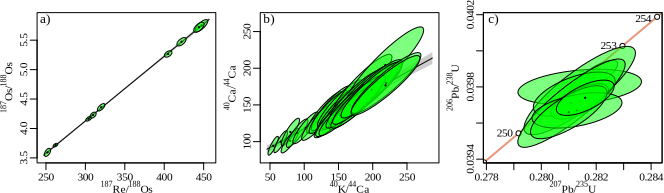
\includegraphics[width=\textwidth]{../figures/errorcorrelation_edited.pdf}
\captionof{figure}{ Examples of correlated uncertainties shown as
  confidence ellipses in a) Re--Os and b) K--Ca isochron and c)
  Wetherill U--Pb concordia space.\\}
\label{fig:errorcorrelation}

For some geochronometers, the error correlations can be reduced by
recasting the isotopes into two new ratios $z/y$ vs. $x/y$. If $y$ is
measured more precisely than $x$ and $z$, then this reduces the
spurious correlation coefficient. For example, revisiting the earlier
Re--Os example:
\[
  \noindent r\left[\frac{{}^{188}\mbox{Os}}{{}^{187}\mbox{Os}},
                   \frac{{}^{187}\mbox{Re}}{{}^{187}\mbox{Os}}\right]
  =
  \frac{
    \left(\frac{10}{2000}\right)^2
  }{
    \sqrt{\left(\frac{100}{30,000}\right)^2 +
      \left(\frac{10}{2000}\right)^2}
    \sqrt{\left(\frac{2}{200}\right)^2 +
      \left(\frac{10}{2000}\right)^2}
  }
  = 0.37
\]

The same change of variables can be applied to other geochronometers
as well:\\

\noindent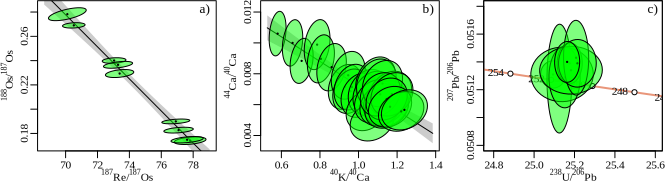
\includegraphics[width=\textwidth]{../figures/inverrorcorrelation_edited.pdf}
\captionof{figure}{ Recasting the data of
  Figure~\ref{fig:errorcorrelation} into an inverse ratio form reduces
  the error correlations for the Re--Os, K--Ca and U--Pb data.\\}
\label{fig:inverrorcorrelation}

Given a data table of conventional ratios ($X=x/z$ and $Y=y/z$), it is
possible to calculate the inverse ratios ($X'=x/y$ and $Y'=z/y$),
their uncertainties ($s[X']$ and $s[Y']$) and error correlations
($r[X',Y']$) using the following equations:

\begin{equation}
  \begin{cases}
    X' = \frac{X}{Y} \\
    Y' = \frac{1}{Y} \\
    \left(\frac{s[X']}{X'}\right)^2 =
    \left(\frac{s[X]}{X}\right)^2 -
    2 r[X,Y]\left(\frac{s[X]}{X}\right)\left(\frac{s[Y]}{Y}\right) +
    \left(\frac{s[Y]}{Y}\right)^2 \\
    \left(\frac{s[Y']}{Y'}\right)^2 = \left(\frac{s[Y]}{Y}\right)^2 \\
    r[X'Y'] =
    \left(\frac{X'}{s[X']}\right)
    \left[
    \left(\frac{Y}{s[Y]}\right) -
    r[X,Y]\left(\frac{X}{s[X]}\right)
    \right]
  \end{cases}
  \label{eq:transformation}
\end{equation}

This transformation is perfectly symmetric in the sense that it can
also be used to convert inverse isochron ratios to conventional
ones. To do this, it suffices to swap $X'$ and $Y'$ for $X$ and $Y$
and vice versa. \texttt{IsoplotR} carries out these conversions on the
fly. So if a data file provides the isotopic composition as
conventional ratios, then it is possible to plot the data as inverse
ratios without worrying about the details of the conversion.

\section{Linear regression}
\label{sec:regression}

As briefly discussed in Chapter~\ref{ch:intro2PD}, isochrons are an
important instrument of high precision, high accuracy geochronology.
Given several aliquots from a single sample, they allow the
non-radiogenic component of the daughter nuclide to be quantified and
separated from the radiogenic component. A conventional isochron is
obtained by fitting a straight line through the conventional isochron
ratios introduced in Section~\ref{sec:errorcorrelations}. The slope
and intercept then yield the radiogenic daughter-parent ratio and the
non-radiogenic daughter composition, respectively
\citep{nicolaysen1961}. In its simplest form, isochrons are fitted by
ordinary least squares regression.\\

Consider a set of $n$ bivariate data points $x =
\{x_1,x_2,\ldots,x_n\}$ and $y = \{y_1,y_2,\ldots,y_n\}$.  The best
fit straight line through these data can be found by minimising the
sum of the squared residuals:
\begin{equation}
  S = \sum\limits_{i=1}^{n}\left( y_i - a - b x_i \right)^2
  \label{eq:S}
\end{equation}

\noindent where $a$ is the intercept and $b$ the slope. However this
method does not take into account the analytical uncertainties of the
isotopic ratio measurements. In a first step, let us consider the
situation where only the dependent variable ($y$) is affected by
significant analytical uncertainty, and let $s[y] =
\{s[y_1],s[y_2],\ldots,s[y_n]\}$ be the corresponding standard
errors. Then the least squares criterion can be modified to create a
weighted regression algorithm:
\begin{equation}
  S_w = \sum\limits_{i=1}^{n}\left( \frac{y_i - a - b x_i}{s[y_i]} \right)^2
  \label{eq:Swtd}
\end{equation}

Alternatively (and equivalently), the best fit line can also be
obtained by maximising the log-likelihood:
\begin{equation}
  \mathcal{LL} = - \sum\limits_{i=1}^{n} \ln\left(2 \pi s[y_i] \right)
  - \frac{S_w}{2}
  \label{eq:L}
\end{equation}

To illustrate the usefulness of the weighted regression algorithm,
consider a simple three-point example. Let $\boldsymbol{x} = \{10, 20,
40\}$ and $\boldsymbol{y} = \{20,30,50\}$ be the \emph{true} x- and
y-coordinates of the three points\footnote{In the remainder of this
  paper, bold face will be used to mark the true values, whereas
  normal face will be used to mark the actual measurements (i.e. the
  true value plus some random analytical uncertainty).}. It is easy to
see that these fall on a perfect line with intercept $\boldsymbol{a} =
10$ and slope $\boldsymbol{b} = 1$. Let $s[\boldsymbol{y}] =
\{1,1,10\}$ be the analytical uncertainties of \textbf{y}, so that the
third point is ten times less precise than the first two. Further let
$y = \{20,30,60\}$ be a random realisation of \textbf{y}.  Then the
best ordinary least squares fit through $x = \boldsymbol{x}$ and $y$
has an intercept of $a = 5.0$ and a slope of $b = 1.36$. This poor
result is strongly influenced by the third, least precise data
point. Subjecting the same dataset to weighted linear regression
yields $a = 9.4$ and $b = 1.04$. This is a far more accurate result
(Figure~\ref{fig:regression}.a).\\

In isochron regression, it is typical for not only $y$ but also $x$ to
be affected by analytical uncertainty. In this case, the best fit line
can be found by modifying the likelihood function
\citep{titterington1979, york1969, york2004}:

\begin{equation}
  \mathcal{LL}_y = 
  -\frac{1}{2} \sum\limits_{i=1}^{n}
  \ln\left(2 \pi |\Sigma_i| \right)
  -\frac{1}{2} \sum\limits_{i=1}^{n}
  \left[X_i-\hat{X}_i\right]^T
  \Sigma_i^{-1}
  \left[X_i-\hat{X}_i\right]
  \label{eq:Ly}
\end{equation}

\noindent where

\begin{equation}
  X_i = \left[
    \begin{array}{@{}c@{}}
      x_i\\
      y_i\\
    \end{array}
    \right]
  \mbox{~,~}
  \hat{X}_i = \left[
    \begin{array}{@{}c@{}}
      \hat{x}_i \\
      a + b \hat{x}_i
    \end{array}
    \right]
  \mbox{~and~}
  \Sigma_i = \left[
    \begin{array}{@{}cc@{}}
      s[x_i]^2 & s[x_i,y_i] \\
      s[x_i,y_i] & s[y_i]^2
    \end{array}
    \right]
\end{equation}

\noindent where $\hat{x}_i$ are the \emph{estimated} values of
$\mathbf{x}_i$ for any value of $a$ or $b$. $s[x_i,y_i]$ is the
covariance of the $i$\textsuperscript{th} measurement's x- and
y-uncertainties. To illustrate the importance of these covariance
terms, consider a second three-point example:

\begin{center}
\begin{tabular}{cccccc}
  $i$ & \textbf{x} & $s[\boldsymbol{x}]$ & \textbf{y} &
  $s[\boldsymbol{y}]$ & $s[\boldsymbol{x}_i,\boldsymbol{y}_i]$ \\
  \hline
  1 & 10 & 1 & 20 & 1 & 0.9 \\
  2 & 20 & 1 & 30 & 1 & 0.9 \\
  3 & 30 & 1 & 40 & 1 & -0.9
\end{tabular}
\end{center}

\noindent which again defines a straight line with intercept $a = 10$
and slope $b = 1$. Let $x = \{10,20,28\}$ and $y = \{20,30,42\}$ be a
random realisation of \textbf{x} and \textbf{y}. Suppose that we
ignored or did not know the covariance terms. In that case the
ordinary and weighted regression algorithms would yield the same
outcome because all the samples have the same standard errors ($s[x_i]
= s[y_i] = 1$ for all $i$). The resulting intercept and slope would
then be $a = 7.2$ and $b = 1.21$. However, if we do take into account
the covariances, then the maximum likelihood algorithm yields $a =
9.3$ and $b = 1.05$, which is much closer to the true values of
$\boldsymbol{a} = 10$ and $\boldsymbol{b} = 1$
(Figure~\ref{fig:regression}.b).

\begin{center}
\noindent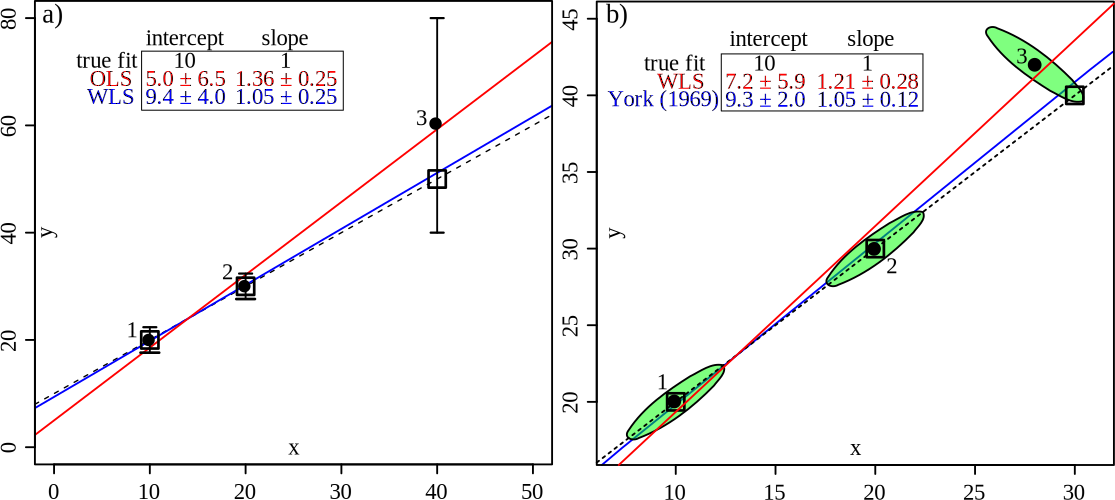
\includegraphics[width=.85\textwidth]{../figures/regression.pdf}
\captionof{figure}{Illustration of the benefits of error-weighted
  linear regression.  The black squares mark the true
  (x,y)-coordinates of three samples drawn from a (dashed) line with
  intercept $\boldsymbol{a} = 10$ and slope $\boldsymbol{b} = 1$. The
  black dots mark random realisations of these samples, given Gaussian
  uncertainties with uncertainties shown as 95\% confidence bars or
  ellipses. a) three samples with analytical uncertainty in the
  y-variable only. The ordinary least squares fit ignoring these
  uncertainties is shown in red ($a = 5.0, b = 1.36$), the weighted
  least squares fit in blue ($a = 9.4, b = 1.04$). b) three samples
  with correlated uncertainties in both the x- and y-variable.
  Ignoring the error correlations yields the red fit ($a = 7.2, b =
  1.21$). Accounting for the error correlations produces the blue fit
  ($a = 9.3, b = 1.05$).}
\label{fig:regression}
\end{center}

\section{The mean square of weighted deviates (MSWD)}
\label{sec:mswd}

The extent to which the observed scatter in the data around the best
fit isochron line can be explained by the analytical uncertainties can
be assessed using a chi-square test.  To this end, we define the
chi-square statistic as:
\begin{equation}
  \chi_{stat}^2 = \sum\limits_{i=1}^{n} \left[X_i - \hat{X}_i\right]^T
  \Sigma_i^{-1} \left[X_i - \hat{X}_i\right]
  \label{eq:Chi2}
\end{equation}

\noindent in which we recognise the second term of
Equation~\ref{eq:Ly}, which is the matrix formulation of the sum of
squares. For example, consider the dataset shown in
Figure~\ref{fig:regression}.b:

\begin{center}
\begin{tabular}{cccccccc}
  $i$ & $x$ & $s[x]$ & $y$ & $s[y]$ &
  $s[\hat{x}_i,\hat{y}_i]$ & $\hat{x}$ & $\hat{y}$ \\
  \hline
  1 & 10 & 1 & 20 & 1 &  0.9 & 10.13 & 19.96 \\
  2 & 20 & 1 & 30 & 1 &  0.9 & 19.75 & 30.09 \\
  3 & 28 & 1 & 42 & 1 & -0.9 & 29.58 & 40.43
\end{tabular}
\end{center}

\noindent where the $\hat{x}$ and $\hat{y}$ values were estimated
using the \citet{york1969} algorithm. Then
\[
\begin{split}
\chi_{stat}^2 = &
\left[
  \begin{array}{cc}
    (10 - 10.13) & (20 - 19.96)\\
  \end{array}
  \right]
\left[
  \begin{array}{cc}
    1^2 & 0.9^2 \\
    0.9^2 & 1^2
  \end{array}
  \right]^{-1}
\left[\begin{array}{c}
    (10 - 10.13)\\
    (20 - 19.96)
  \end{array}
  \right] \\
+ & \left[
  \begin{array}{cc}
    (20 - 19.75) & (30 - 30.09)\\
  \end{array}
  \right]
\left[
  \begin{array}{cc}
    1^2 & 0.9^2 \\
    0.9^2 & 1^2
  \end{array}
  \right]^{-1}
\left[\begin{array}{c}
    (20 - 19.75) \\
    (30 - 30.09)
  \end{array}
  \right] \\
+ & \left[
  \begin{array}{cc}
    (28 - 29.58) & (42 - 40.43)\\ 
  \end{array}
  \right]
\left[
  \begin{array}{cc}
    1^2 & 0.9^2 \\
    0.9^2 & 1^2
  \end{array}
  \right]^{-1}
\left[\begin{array}{c}
    (28 - 29.58) \\
    (42 - 40.43)
  \end{array}
  \right] = 3.32
\end{split}
\]

We can compare this value with a chi-square distribution with $df =
(k-1) n - k$ degrees of freedom, where $k$ is the dimensionality of
the linear fit. In the case of our example dataset, $k=2$ and $n=3$,
so $df=1$. The \textbf{p-value} is defined as the probability of
observing a value greater than $\chi_{stat}^2$ under this
distribution:

\noindent\begin{minipage}[t]{.7\textwidth}
\strut\vspace*{-\baselineskip}\newline
\includegraphics[width=\textwidth]{../figures/chi2.pdf}
\end{minipage}
\begin{minipage}[t]{.3\textwidth}
  \captionof{figure}{Chi-square distribution with 1 degree of freedom.
    The p-value for an outcome of $\chi_{stat}^2=3.32$ is the integral
    of the black area.}
  \label{fig:chi2}
\end{minipage}

If the p-value falls below a cutoff value of 0.05, say, then this
indicates that the data are `overdispersed' with respect to the formal
analytical uncertainties around the best-fit line. In contrast,
p-values that are much greater than 0.95 are indicative of
`underdispersed' data, possibly reflecting overestimated analytical
uncertainties.\\

An alternative way to assess the degree of over- or underdispersion is
by dividing the chi-square statistic $\chi^2_{stat}$ by the number of
degrees of freedom $df$. The resulting numerical value is called the
`Mean Square of the Weighted Deviates' \citep[MSWD,][]{mcintyre1966}
by geochronologists, but is known as the `reduced chi-square
statistic' elsewhere. For sufficiently large samples and, hence,
degrees of freedom, the distribution of the MSWD statistic converges
to a normal distribution with a mean of 1. However for small samples
there is a comparatively greater probability of obtaining an MSWD
value that is greater or smaller than 1:

\noindent\begin{minipage}[t]{.7\textwidth}
\strut\vspace*{-\baselineskip}\newline
\includegraphics[width=\textwidth]{../figures/mswd.pdf}
\end{minipage}
\begin{minipage}[t]{.3\textwidth}
  \captionof{figure}{Expected distribution of the MSWD for different
    degrees of freedom. With increasing sample size, the distribution
    of the MSWD converges to a normal distribution with mean 1.}
  \label{fig:mswd}
\end{minipage}

The MSWD is a very useful device to assess the degree to which the
observed scatter of the data around the best fit can be explained by
the analytical uncertainties. Three scenarios are possible:

\begin{enumerate}
  \item If the analytical uncertainties alone explain the total
    scatter around the true mean, then the MSWD is expected to take on
    a value of $\approx{1}$.
\item Data sets that exhibit MSWD values close to zero are said to be
  ``underdispersed'' with respect to the analytical
  uncertainties. This indicates some problem with the error
  propagation, which is often due to undetected systematic effects.
\item Finally, MSWD values $>1$ can often be attributed to some form
  of geological dispersion. This overdispersion carries geological
  significance.
\end{enumerate}

\noindent\begin{minipage}[t]{.5\textwidth}
\strut\vspace*{-\baselineskip}\newline
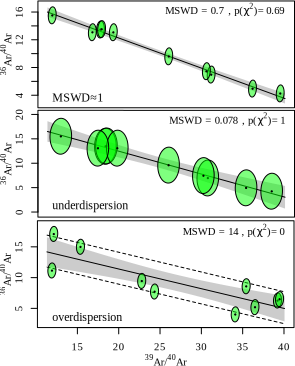
\includegraphics[width=\textwidth]{../figures/ArArMSWD.pdf}
\end{minipage}
\begin{minipage}[t]{.5\textwidth}
  \vspace{-20pt}
  \captionof{figure}{Three different synthetic
    \textsuperscript{40}Ar/\textsuperscript{39}Ar data sets shown as
    inverse isochron plots. The analytical uncertainties are shown as
    95\% error ellipses. The grey band represents a 95\% confidence
    envelope for the best fit line using the \citet{york1969}
    algorithm. Each of the data sets consists of 10 aliquots that are
    affected by a combination of analytical and geological
    dispersion. The relative importance of these two sources of
    scatter can be assessed using the mean square of weighted deviates
    (MSWD) and the p-value of the chi-square test. The case where
    MSWD$\approx{1}$ is the easiest to interpret: it means that the
    scatter of the data around the best fit line can be completely
    explained by the analytical uncertainty. The case where MSWD$<{1}$
    may seem like a good outcome but it is in fact a bad one because
    it indicates that there may be a problem with the error
    propagation. A high p-value or low MSWD may happen once but red
    flags should go up if all samples in a study show this type of
    behaviour. Finally the case where MSWD$>{1}$ is not good or bad
    but `interesting'. This requires further investigation as
    discussed in Section~\ref{sec:overdispersion}.  }
  \label{fig:ArArMSWD}
\end{minipage}

\section{Dealing with overdispersion}
\label{sec:overdispersion}

\texttt{IsoplotR} offers three strategies (`models') to deal with
overdispersed datasets:

\begin{enumerate}
\item inflate the analytical uncertainties until MSWD=1;
\item ignore the analytical uncertainties;
\item quantify the overdispersion.
\end{enumerate}

Let us consider the simple case of a 2-dimensional dataset
$\{x_1,y_1\},\ldots,\{x_i,y_i\},\ldots,\{x_n,y_n\}$.  Data are
overdispersed with respect to the analytical uncertainties if:

\[
\mathrm{MSWD} \equiv
\sum\limits_{i=1}^n X_i~\Omega_i X_i^T / df > 1
\]

\noindent with

\[
X_i = \left[
  \begin{array}{cc}
    (x_i - \hat{x}_i) &  (y_i - \hat{y}_i)
  \end{array}
  \right],
\]

\noindent where $\hat{x}_i$ and $\hat{y}_i$ are the fitted values, and

\[
\Omega_i \equiv
\left[
  \begin{array}{cc}
    s[x_i]^2 & cov(x_i,y_i) \\
    cov(x_i,y_i) & s[y_i]^2
  \end{array}
\right]^{-1}
\]

\texttt{IsoplotR} provides three alternative strategies (`models') to
deal with overdispersed data. A first way (`model-1') to account for
overdispersion is to inflate all analytical uncertainties by a common
\emph{factor} $f$, which is chosen so as to reduce the MSWD to unity:

\[
\sum\limits_{i=1}^{n} X_i~\Omega_{i,f} X_i^T / df = 1
\]

\noindent with

\[
\Omega_{i,f}
\equiv
\left[
  \begin{array}{cc}
    f^2s[x_i]^2 & f^2cov(x_i,y_i) \\
    f^2cov(x_i,y_i) & f^2s[y_i]^2
  \end{array}
\right]^{-1}
= \Omega_i/f^2
\]

\noindent from which it is easy to show that $f=\sqrt{\mathrm{MSWD}}$.\\

A second option (`model-2') for dealing with overdispersion is to
simply ignore the analytical uncertainties and perform an ordinary
least squares regression. This option is offered for the sake of
completeness but is inherently flawed, because (1) its results may
differ depending on which ratio is chosen as the dependent variable;
(2) it assumes that only the dependent variable is subject to scatter;
which results in (3) unreliable error calculations
\citep[][p. 648]{ludwig2003b}. \\

Finally, a third option (`model-3') is to attribute the overdispersion
to geological scatter in the ages or in the non-radiogenic isotope
composition. The latter hypothesis can be formalised as follows:

\[
\sum\limits_{i=1}^{n} X_i~\Omega_{i,\omega} X_i^T / df = 1
\]

\noindent with

\[
\Omega_{i,\omega} \equiv
\left[
  \begin{array}{cc}
    s[x_i]^2 & cov(x_i,y_i) \\
    cov(x_i,y_i) &  s[y_i]^2 + \omega^2
  \end{array}
\right]^{-1}
\]

\noindent where $\omega$ is the overdispersion \emph{term}, which can
be found iteratively. This term has geological significance and is
reported separately by \texttt{IsoplotR}. The third strategy is
arguably the most sensible one, because geological scatter is a very
common phenomenon.  For example, not all aliquots in a multi-mineral
Rb-Sr isochron may have formed with exactly the same initial
\textsuperscript{87}Sr/\textsuperscript{86}Sr ratio
\citep{mcintyre1966}. As the analytical precision of mass
spectrometers has increased over the years, geochronologists' ability
to detect even the smallest amount of geological dispersion has
steadily grown as well. It is reasonable to assume that this trend
will continue into the future, and that overdispersed datasets will
become ever more common.\\

It is important to note that the overdispersion of geochronological
datasets contains meaningful geological information. For example, the
dispersion of igneous zircon U-Pb dates bears information on the
magmatic residence time of these crystals \citep{matzel2006,
  rioux2012}.  Thus, the increasing prevalence of overdispersed
datasets should be seen as a positive trend rather than a nuisance.

\printbibliography[heading=subbibliography]

\end{refsection}
